% Aberdeen style guide should be followed when using this
% layout. Their template powerpoint slide is used to extract the
% Aberdeen color and logo but is otherwise ignored (it has little or
% no formatting in it anyway).
%
% http://www.abdn.ac.uk/documents/style-guide.pdf

%%%%%%%%%%%%%%%%%%%% Document Class Settings %%%%%%%%%%%%%%%%%%%%%%%%%
% Pick if you want slides, or draft slides (no animations)
%%%%%%%%%%%%%%%%%%%%%%%%%%%%%%%%%%%%%%%%%%%%%%%%%%%%%%%%%%%%%%%%%%%%%%
%Normal document mode%
\documentclass[10pt,compress]{beamer}
%Draft or handout mode
%\documentclass[10pt,compress,handout]{beamer}
%\documentclass[10pt,compress,handout,ignorenonframetext]{beamer}

%%%%%%%%%%%%%%%%%%%% General Document settings %%%%%%%%%%%%%%%%%%%%%%%
% These settings must be set for each presentation
%%%%%%%%%%%%%%%%%%%%%%%%%%%%%%%%%%%%%%%%%%%%%%%%%%%%%%%%%%%%%%%%%%%%%%
\newcommand{\shortname}{jefferson.gomes@abdn.ac.uk}
\newcommand{\fullname}{Dr Jeff Gomes}
\institute{School of Engineering}
\newcommand{\emailaddress}{}%jefferson.gomes@abdn.ac.uk}
\newcommand{\logoimage}{../FigBanner/UoAHorizBanner}
\title{Heat, Mass and Momentum Conservation -- Thermodynamics2 (EM40JK/EX3030)}
\subtitle{Transient Heat Transfer}
%\subtitle{Module 1.1: Review of Thermodynamics}
\date[ ]{ }

%%%%%%%%%%%%%%%%%%%% Template settings %%%%%%%%%%%%%%%%%%%%%%%%%%%%%%%
% You shouldn't have to change below this line, unless you want to.
%%%%%%%%%%%%%%%%%%%%%%%%%%%%%%%%%%%%%%%%%%%%%%%%%%%%%%%%%%%%%%%%%%%%%%
\usecolortheme{whale}
\useoutertheme{infolines}

% Use the fading effect for items that are covered on the current
% slide.
\beamertemplatetransparentcovered

% We abuse the author command to place all of the slide information on
% the title page.
\author[\shortname]{%
  \fullname\\\ttfamily{\emailaddress}
}


%At the start of every section, put a slide indicating the contents of the current section.
\AtBeginSection[] {
  \begin{frame}
    \frametitle{Section Outline}
    \tableofcontents[currentsection]
  \end{frame}
}

% Allow the inclusion of movies into the Presentation! At present,
% only the Okular program is capable of playing the movies *IN* the
% presentation.
\usepackage{multimedia}
\usepackage{animate}

%% Handsout -- comment out the lines below to create handstout with 4 slides in a page with space for comments
\usepackage{handoutWithNotes}

\mode<handout>
{
\usepackage{pgf,pgfpages}

\pgfpagesdeclarelayout{2 on 1 boxed with notes}
{
\edef\pgfpageoptionheight{\the\paperheight} 
\edef\pgfpageoptionwidth{\the\paperwidth}
\edef\pgfpageoptionborder{0pt}
}
{
\setkeys{pgfpagesuselayoutoption}{landscape}
\pgfpagesphysicalpageoptions
    {%
        logical pages=4,%
        physical height=\pgfpageoptionheight,%
        physical width=\pgfpageoptionwidth,%
        last logical shipout=2%
    } 
\pgfpageslogicalpageoptions{1}
    {%
    border code=\pgfsetlinewidth{1pt}\pgfstroke,%
    scale=1,
    center=\pgfpoint{.25\pgfphysicalwidth}{.75\pgfphysicalheight}%
    }%
\pgfpageslogicalpageoptions{2}
    {%
    border code=\pgfsetlinewidth{1pt}\pgfstroke,%
    scale=1,
    center=\pgfpoint{.25\pgfphysicalwidth}{.25\pgfphysicalheight}%
    }%
\pgfpageslogicalpageoptions{3}
    {%
    border shrink=\pgfpageoptionborder,%
    resized width=.7\pgfphysicalwidth,%
    resized height=.5\pgfphysicalheight,%
    center=\pgfpoint{.75\pgfphysicalwidth}{.29\pgfphysicalheight},%
    copy from=3
    }%
\pgfpageslogicalpageoptions{4}
    {%
    border shrink=\pgfpageoptionborder,%
    resized width=.7\pgfphysicalwidth,%
    resized height=.5\pgfphysicalheight,%
    center=\pgfpoint{.75\pgfphysicalwidth}{.79\pgfphysicalheight},%
    copy from=4
    }%

\AtBeginDocument
    {
    \newbox\notesbox
    \setbox\notesbox=\vbox
        {
            \hsize=\paperwidth
            \vskip-1in\hskip-1in\vbox
            {
                \vskip1cm
                Notes\vskip1cm
                        \hrule width\paperwidth\vskip1cm
                    \hrule width\paperwidth\vskip1cm
                        \hrule width\paperwidth\vskip1cm
                    \hrule width\paperwidth\vskip1cm
                        \hrule width\paperwidth\vskip1cm
                    \hrule width\paperwidth\vskip1cm
                    \hrule width\paperwidth\vskip1cm
                    \hrule width\paperwidth\vskip1cm
                        \hrule width\paperwidth
            }
        }
        \pgfpagesshipoutlogicalpage{3}\copy\notesbox
        \pgfpagesshipoutlogicalpage{4}\copy\notesbox
    }
}
}

%\pgfpagesuselayout{2 on 1 boxed with notes}[letterpaper,border shrink=5mm]
%\pgfpagesuselayout{2 on 1 boxed with notes}[letterpaper,border shrink=5mm]



%%%%% Color settings
\usepackage{color}
%% The background color for code listings (i.e. example programs)
\definecolor{lbcolor}{rgb}{0.9,0.9,0.9}%
\definecolor{UoARed}{rgb}{0.64706, 0.0, 0.12941}
\definecolor{UoALight}{rgb}{0.85, 0.85, 0.85}
\definecolor{UoALighter}{rgb}{0.92, 0.92, 0.92}
\setbeamercolor{structure}{fg=UoARed} % General background and higlight color
\setbeamercolor{frametitle}{bg=black} % General color
\setbeamercolor{frametitle right}{bg=black} % General color
\setbeamercolor{block body}{bg=UoALighter} % For blocks
\setbeamercolor{structure}{bg=UoALight} % For blocks
% Rounded boxes for blocks
\setbeamertemplate{blocks}[rounded]

%%%%% Font settings
% Aberdeen requires the use of Arial in slides. We can use the
% Helvetica font as its widely available like so
% \usepackage{helvet}
% \renewcommand{\familydefault}{\sfdefault}
% But beamer already uses a sans font, so we will stick with that.

% The size of the font used for the code listings.
\newcommand{\goodsize}{\fontsize{6}{7}\selectfont}

% Extra math packages, symbols and colors. If you're using Latex you
% must be using it for formatting the math!
\usepackage{amscd,amssymb} \usepackage{amsfonts}
\usepackage[mathscr]{eucal} \usepackage{mathrsfs}
\usepackage{latexsym} \usepackage{amsmath} \usepackage{bm}
\usepackage{amsthm} \usepackage{textcomp} \usepackage{eurosym}
% This package provides \cancel{a} and \cancelto{a}{b} to "cancel"
% expressions in math.
\usepackage{cancel}

\usepackage{comment} 

% Get rid of font warnings as modern LaTaX installations have scalable
% fonts
\usepackage{type1cm} 

%\usepackage{enumitem} % continuous numbering throughout enumerate commands

% For exact placement of images/text on the cover page
\usepackage[absolute]{textpos}
\setlength{\TPHorizModule}{1mm}%sets the textpos unit
\setlength{\TPVertModule}{\TPHorizModule} 

% Source code formatting package
\usepackage{listings}%
\lstset{ backgroundcolor=\color{lbcolor}, tabsize=4,
  numberstyle=\tiny, rulecolor=, language=C++, basicstyle=\goodsize,
  upquote=true, aboveskip={1.5\baselineskip}, columns=fixed,
  showstringspaces=false, extendedchars=true, breaklines=false,
  prebreak = \raisebox{0ex}[0ex][0ex]{\ensuremath{\hookleftarrow}},
  frame=single, showtabs=false, showspaces=false,
  showstringspaces=false, identifierstyle=\ttfamily,
  keywordstyle=\color[rgb]{0,0,1},
  commentstyle=\color[rgb]{0.133,0.545,0.133},
  stringstyle=\color[rgb]{0.627,0.126,0.941}}

% Allows the inclusion of other PDF's into the final PDF. Great for
% attaching tutorial sheets etc.
\usepackage{pdfpages}
\setbeamercolor{background canvas}{bg=}  

% Remove foot note horizontal rules, they occupy too much space on the slide
\renewcommand{\footnoterule}{}

% Force the driver to fix the colors on PDF's which include mixed
% colorspaces and transparency.
\pdfpageattr {/Group << /S /Transparency /I true /CS /DeviceRGB>>}

% Include a graphics, reserve space for it but
% show it on the next frame.
% Parameters:
% #1 Which slide you want it on
% #2 Previous slides
% #3 Options to \includegraphics (optional)
% #4 Name of graphic
\newcommand{\reserveandshow}[4]{%
\phantom{\includegraphics<#2|handout:0>[#3]{#4}}%
\includegraphics<#1>[#3]{#4}%
}

\newcommand{\frc}{\displaystyle\frac}
\newcommand{\red}{\textcolor{red}}
\newcommand{\blue}{\textcolor{blue}}
\newcommand{\green}{\textcolor{green}}
\newcommand{\purple}{\textcolor{purple}} 

\begin{document}

% Title page layout
\begin{frame}
  \titlepage
  \vfill%
  \begin{center}
    \includegraphics[clip,width=0.8\textwidth]{\logoimage}
  \end{center}
\end{frame}

% Table of contents
%\frame{ \frametitle{Slides Outline}
%  \tableofcontents
%}


%%%%%%%%%%%%%%%%%%%% The Presentation Proper %%%%%%%%%%%%%%%%%%%%%%%%%
% Fill below this line with \begin{frame} commands! It's best to
% always add the fragile option incase you're going to use the
% verbatim environment.
%%%%%%%%%%%%%%%%%%%%%%%%%%%%%%%%%%%%%%%%%%%%%%%%%%%%%%%%%%%%%%%%%%%%%%

%%%
%%% SECTION
%%%
\section{Introduction} 


%%% SUBSECTION
\subsection{Objectives}

%%%
%%% Slide
%%%
\begin{frame}
 \frametitle{Aims and Objectives}
   \begin{enumerate}
     \item Lumped system analysis
     \item Transient heat conduction
%• Assess when the spatial variation of temperature is negligible, and temperature varies nearly uniformly with time, making the simplified lumped system analysis applicable,
% • Obtain analytical solutions for transient one-dimensional conduction problems in rectangular, cylindrical, and spherical geometries using the method of separation of variables, and understand why a one-term solution is usually a reasonable approximation,
% • Solve the transient conduction problem in large mediums using the similarity variable, and predict the variation of temperature with time and distance from the exposed surface, and
% • Construct solutions for multi-dimensional transient conduction problems using the product solution approach.
   \end{enumerate}
\end{frame}


%%%
%%% SUBSECTION
%%%
\subsection{Bibliography} 

%%%
%%% Slide
%%%
\begin{frame}
 \frametitle{Suggested References}
  Literature relevant for this module:
  \begin{enumerate}[{[}1{]}]
    \item J.P. Holman, `Heat Transfer', 10$^{th}$ Edition (McGraw-Hill): Chapters 4 and 10;
    \item F.P. Incropera, D.P. DeWitt, T.L.Bergman, A.S. Lavine, `introduction to Heat Transfer' (John Willey $\&$ Sons): Chapters 5 and 11.
    \item L. Theodore, `Essential Engineering Calculations Series: Heat Transfer Applications for the Practicing Engineer' (John Willey $\&$ Sons): Chapters 8 and 14.
  \end{enumerate}
\end{frame}
 

%%%
%%%  SECTION
%%%
\section{Unsteady-State Conduction}

%%% SUBSECTION
\subsection{Introduction}

%%%
%%% Slide
%%%
\begin{frame}
 \frametitle{Introduction}
   \begin{columns}
     \begin{column}[l]{0.5\linewidth}
        \begin{center}
          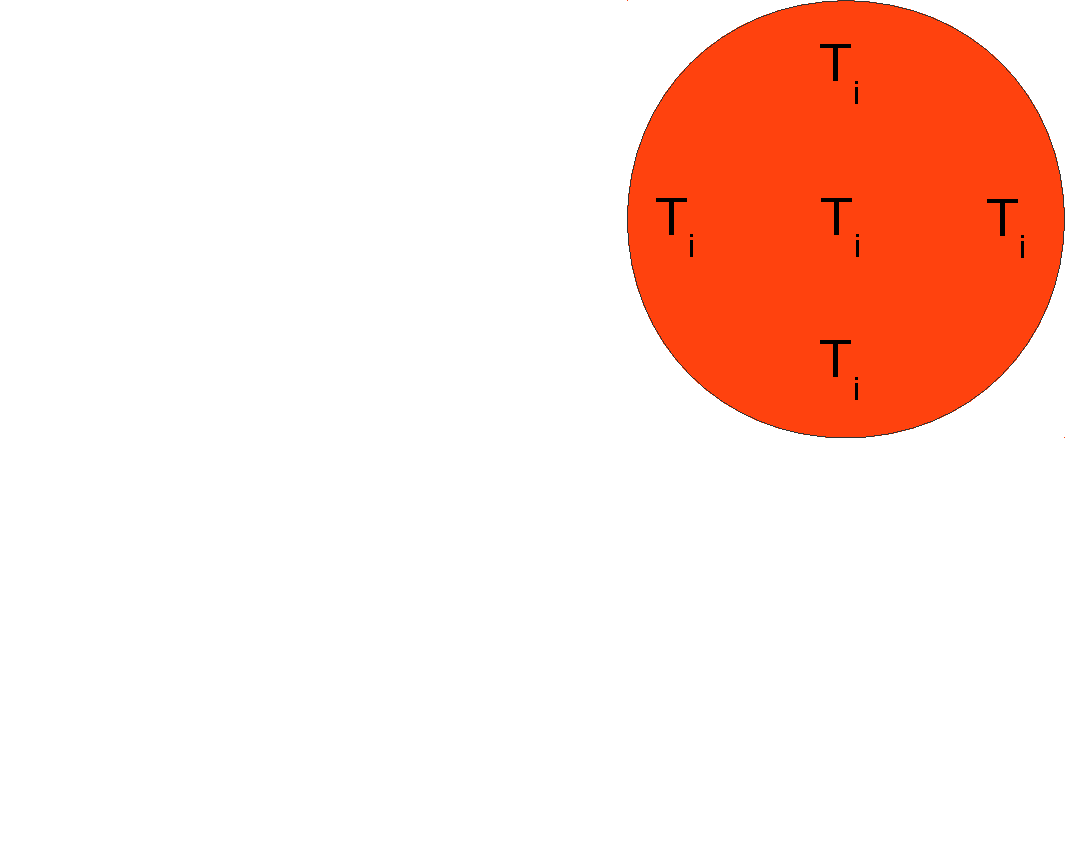
\includegraphics[width=\columnwidth,clip]{./Pics/Lumped1}
        \end{center}
     \end{column}
%
     \begin{column}[l]{0.5\linewidth}
        \begin{enumerate}
           \item<1-> In the study of heat transfer, the simplest case analysis is when bodies are assumed {\it isothermal} and, therefore they can be treated as a \blue{lump} system;
           \item<1-> This means that the temperature of these bodies at any spatial coordinate can be expressed as function of time only, i.e., \blue{$T=T\left(t\right)$};
        \end{enumerate}
     \end{column}     
   \end{columns}
\end{frame}

%%%
%%% SUBSECTION
%%%
\subsection{Lumped Systems}

%%%
%%% Slide
%%%
\begin{frame}
 \frametitle{Thermal Energy Balance}
   \begin{enumerate}
     \item<1-> Let's consider a body of mass \blue{$m$} and arbitrary shape $\left(\text{with area} \blue{A_{s}}\right)$ and temperature \blue{$T$};
     \item<1-> The body is assumed homogeneous and we can consider constant heat capacity at constant pressure, \blue{$C_{p}$}, thermal conductivity, \blue{$\kappa$} and;
     \item<2-> The energy balance of an isothermal body during time interval \blue{$dt$}, subject to constant surrounding temperature \blue{$T_{\infty}$}, can be simplified as,\\
       \begin{center}
        \begin{tabular}{c c c}
           \visible<3->{\blue{Heat transferred into}} & \visible<3->{=} & \visible<4->{\red{Increase of thermal energy}} \\
           \visible<3->{\blue{the body during $dt$}}  &                 & \visible<4->{\red{of the body during $dt$}} \\
                                                      &                 & \\
           \visible<3->{\blue{$\Downarrow$}}          &                 & \visible<4->{\red{$\Downarrow$}}\\
                                                      &                 & \\
           \visible<3->{\blue{$hA_{s}\left(T_{\infty}-T\right)dt$}}& \visible<3->{=} & \visible<4->{\red{$mC_{p}dT$}}
        \end{tabular}
        \end{center} 
      \item<5-> For \blue{$m=\rho V$} (where $\rho$ and $V$ are the density and volume of the body, respectively) and;
      \item<5-> \blue{$dT=d\left(T_{\infty}-T\right)$};
   \end{enumerate}
\end{frame}

%%%
%%% Slide
%%%
\begin{frame}
 \frametitle{Thermal Energy Balance}
   \begin{enumerate}\setcounter{enumi}{5}\scriptsize
     \item<1-> The energy balance,
          \visible<1->{\blue{\begin{equation}
              hA_{s}\left(T_{\infty}-T\right)dt = mC_{p}dT \label{eqn:energybalance}
          \end{equation}}}
     \item<1-> can be rearranged and integrated as (from time \blue{0} to \blue{t}),
          \visible<2->{\begin{eqnarray}
              \frc{d\left(T-T_{\infty}\right)}{T-T_{\infty}} &=& -\frc{hA_{s}}{\rho V C_{p}}dt \nonumber \\
              \ln\frc{T(t)-T_{\infty}}{T_{0}-T_{\infty}} &=& -\frc{hA_{s}}{\rho V C_{p}}t \nonumber \\
              \blue{\frc{T(t)-T_{\infty}}{T_{0}-T_{\infty}}} &\blue{=}& \blue{e^{-bt}} \label{eqn:CharacteristicTime}
          \end{eqnarray}}
          \visible<2->{where \blue{$T_{0}$} is the initial temperature and $b = \frc{hA_{s}}{\rho V C_{p}}$ is the \blue{time constant} with dimension {\bf $\left[\text{time}^{-1}\right]$}.}
     \item<3-> From Eqn.~\ref{eqn:CharacteristicTime}:
        \begin{enumerate}\scriptsize
           \item<3-> We can calculate either the temperature \blue{$T(t)$} of the body at a given time \blue{$t$} or;
           \item<4-> The time \blue{$t$} required for a body to reach temperature \blue{$T(t)$};
           \item<5-> Temperature \blue{$T(t)$} approaches the surrounding temperature \blue{$T_{\infty}$} {\bf exponentially}.
           \item<6-> A large value of \blue{b} indicates a higher rate of temperature decay;
           \item<7-> Finally, \blue{b} is proportional to \blue{$A_{s}$} and inversely proportional to \blue{$m$} and \blue{$C_{p}$} of the body. This means that it takes longer to heat or cool a larger mass, in particular if it also has a large heat capacity.
        \end{enumerate}
   \end{enumerate}
\end{frame}


%%%
%%% Slide
%%%
\begin{frame}
 \frametitle{Convection Heat Transfer}
   \begin{enumerate}%\setcounter{enumi}{5}\scriptsize
     \item<1-> The {\it Newton's law of cooling} can determine the rate of convection heat transfer,
          \visible<1->{\blue{\begin{equation}
              \dot{Q}(t) = hA_{s}\left[T(t) - T_{\infty}\right] \hspace{1cm} \mathbf{(W)}
          \end{equation}}}
     \item<2-> The heat transferred between the body and the surroundings during time \blue{$\Delta t$} is the energy change in the system (i.e., body + surroundings):
          \visible<2->{\begin{equation}
              \dot{Q} = m C_{p}\left[T(t) - T_{\infty}\right] \hspace{1cm} \mathbf{(J)}
          \end{equation}}
     \item<3-> Therefore the maximum heat exchanged between the body and the surroundings is
          \visible<3->{\begin{equation}
              \dot{Q}_{\text{max}} = m C_{p}\left[T_{0} - T_{\infty}\right] \hspace{1cm} \mathbf{(J)}
          \end{equation}}
   \end{enumerate}
\end{frame}



%%%
%%% Slide
%%%
\begin{frame}
 \frametitle{Criteria for Lumped System}
   \begin{enumerate}%\setcounter{enumi}{5}\scriptsize
     \item<1-> The assumption of {\bf lumped system} is not often the most appropriate. With the {\it characteristic length} \blue{$L_{c}=\frc{V}{A_{s}}$};
     \item<2-> We can determine the dimensionless \red{Biot Number (\it{Bi})},
       \begin{equation}
          \visible<2->{\red{Bi} \blue{= \frc{\text{Conduction resistance within the body}}{\text{Convection resistance at the surface}}}} \visible<3->{\blue{= \frc{\frc{L_{c}}{\kappa}}{\frc{1}{h}}} \red{= \frc{h L_{c}}{\kappa}}}
       \end{equation}  
     \item<4-> {\bf Lumped system} analysis assumes {\it uniform temperature distribution} throughout the body;
     \item<4-> This assumption is correct {\bf if} the convection coefficient is small and thermal conductivity is large, i.e.,;
     \item<5-> \blue{The smaller the {\bf Bi}, the more accurate the lumped system analysis,} 
                     \begin{displaymath}
                       \visible<5->{ \red{Bi \leq 0.1}}
                     \end{displaymath}
   \end{enumerate}
\end{frame}

%%%
%%% Slide
%%%
\begin{frame}
 \frametitle{Criteria for Lumped System}
   \begin{enumerate}\setcounter{enumi}{5}\scriptsize
     \item<1-> Example: Two spheres are removed from a furnace and let to cool with air at 25$^{\circ}$C. The spheres are made of copper $\left(\kappa=401$ W.$\left(\text{m.}^{\circ}\text{C}\right)^{-1}\right)$ and coal $\left(\kappa=0.2$ W.$\left(\text{m.}^{\circ}\text{C}\right)^{-1}\right)$.\\

     \visible<2->{kki}

Assume $h=15$ W.$\left(\text{m}^{2}.^{\circ}\text{C}\right)^{-1}$.
under  the influence of hot air with For a copper $\left(\kappa=401$ W.$\left(\text{m.}^{\circ}\text{C}\right)^{-1}\right)$ sphere

The assumption of {\bf lumped system} is not often the most appropriate. With the {\it characteristic length} \blue{$L_{c}=\frc{V}{A_{s}}$};
     \item<2-> We can determine the dimensionless \red{Biot Number (\it{Bi})},
       \begin{equation}
          \visible<2->{\red{Bi} \blue{= \frc{\text{Conduction resistance within the body}}{\text{Convection resistance at the surface}}}} \visible<3->{\blue{= \frc{\frc{L_{c}}{\kappa}}{\frc{1}{h}}} \red{= \frc{h L_{c}}{\kappa}}}
       \end{equation}  
     \item<4-> {\bf Lumped system} analysis assumes {\it uniform temperature distribution} throughout the body;
     \item<4-> This assumption is correct {\bf if} the convection coefficient is small and thermal conductivity is large, i.e.,;
     \item<5-> \blue{The smaller the {\bf Bi}, the more accurate the lumped system analysis,} 
                     \begin{displaymath}
                       \visible<5->{ \red{Bi \leq 0.1}}
                     \end{displaymath}
   \end{enumerate}
\end{frame



%%% SUBSECTION
\subsection{Transient Heat Conduction}


%%%
%%%  SECTION
%%%
\section{Design of Heat Exchangers}

%%% SUBSECTION
\subsection{Introduction}

%%% SUBSECTION
\subsection{Overall Heat Transfer Coefficient Calculations}

%%% SUBSECTION
\subsection{Transient Response of Thermal Energy Storage System}










%%%
%%% Appendix
%%%
%\subsection{Appendix}
%\begin{frame}
%\begin{itemize}
%\item Saturated Water and Steam Tables;
%\item Superheated Steam at Various Pressure and Temperatures;
%\item Units Conversion.
%\end{itemize}
%\end{frame}


%{
%  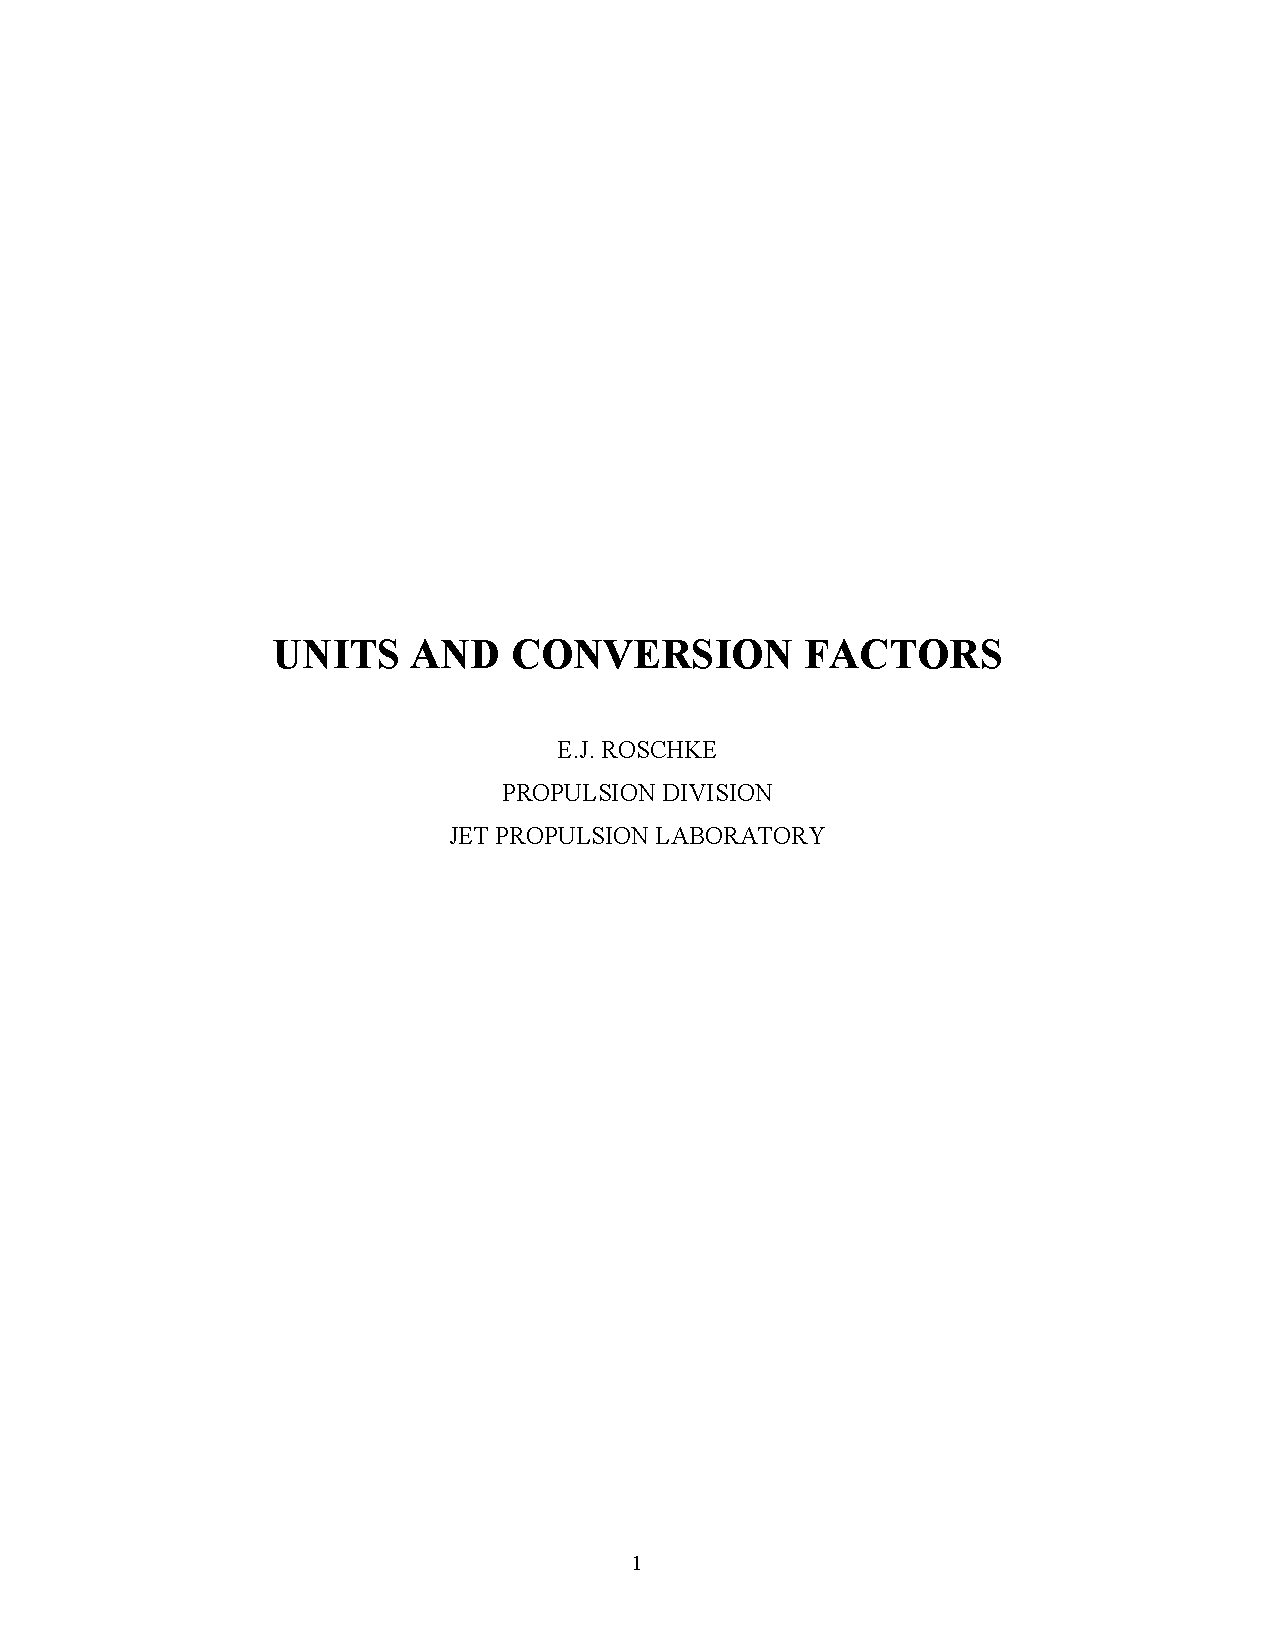
\includepdf[pages=-,fitpaper]{./Pics/Roschke.pdf}
%}


\end{document}
